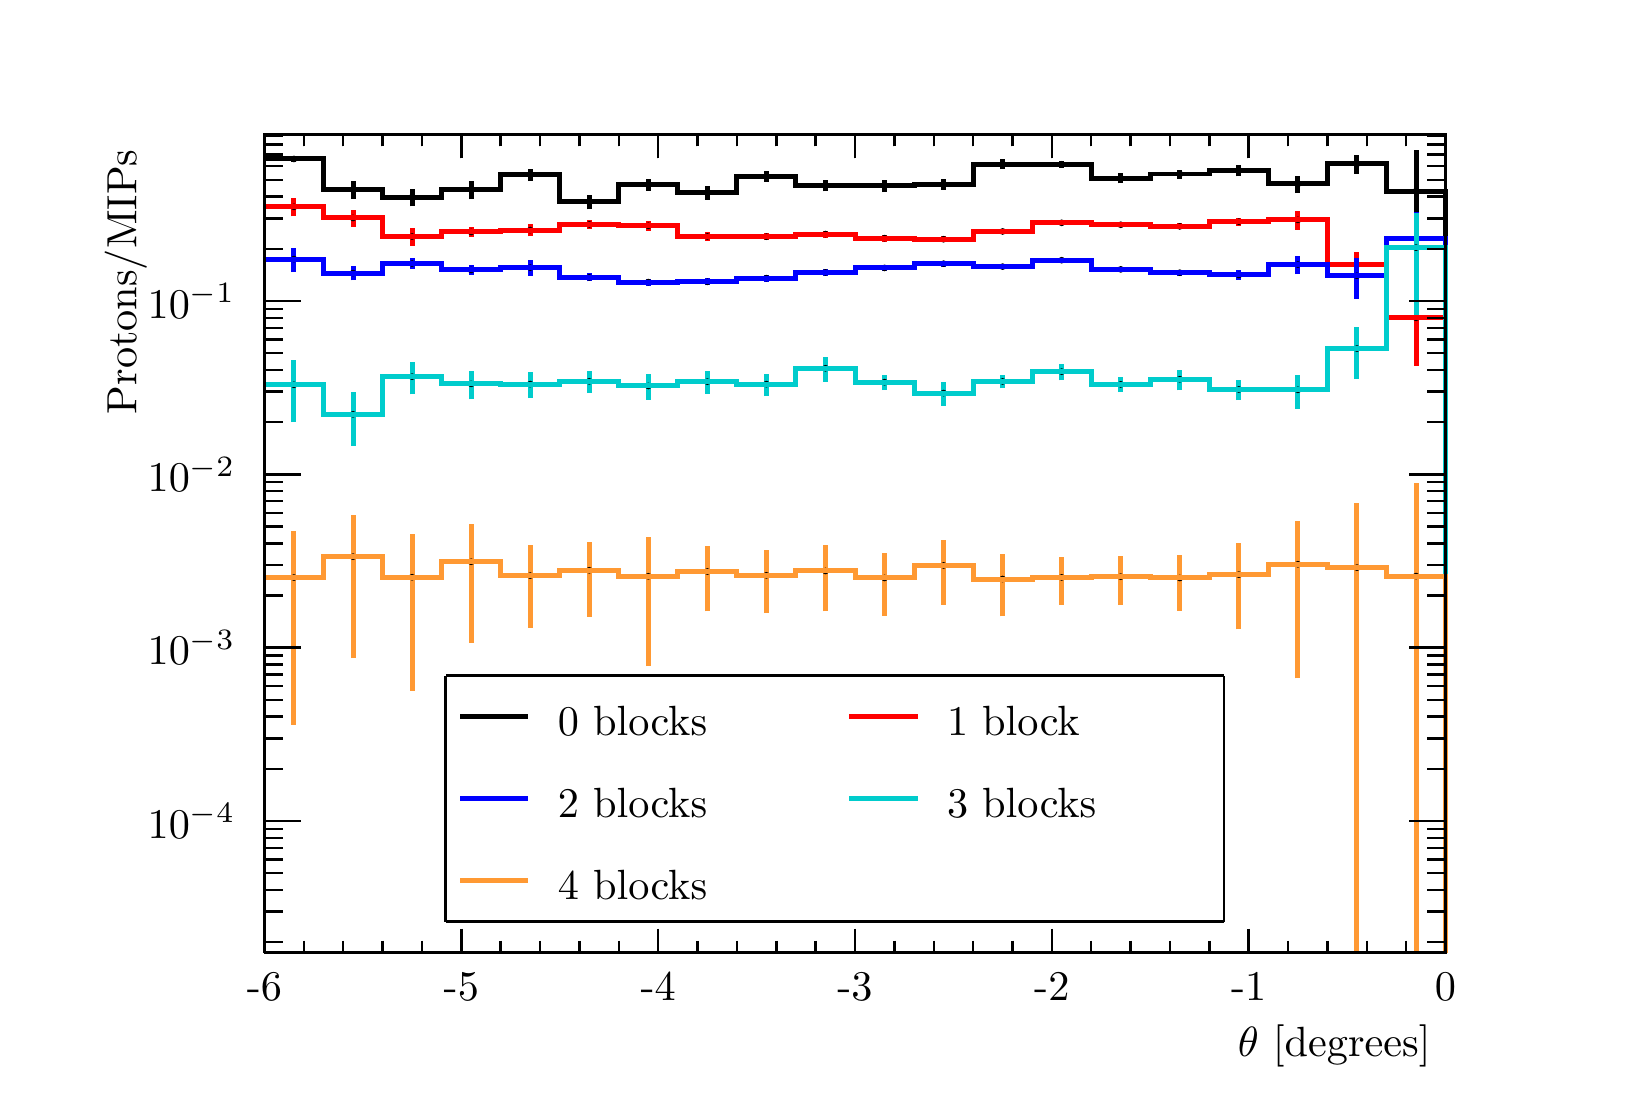
\begin{tikzpicture}
\pgfdeclareplotmark{cross} {
\pgfpathmoveto{\pgfpoint{-0.3\pgfplotmarksize}{\pgfplotmarksize}}
\pgfpathlineto{\pgfpoint{+0.3\pgfplotmarksize}{\pgfplotmarksize}}
\pgfpathlineto{\pgfpoint{+0.3\pgfplotmarksize}{0.3\pgfplotmarksize}}
\pgfpathlineto{\pgfpoint{+1\pgfplotmarksize}{0.3\pgfplotmarksize}}
\pgfpathlineto{\pgfpoint{+1\pgfplotmarksize}{-0.3\pgfplotmarksize}}
\pgfpathlineto{\pgfpoint{+0.3\pgfplotmarksize}{-0.3\pgfplotmarksize}}
\pgfpathlineto{\pgfpoint{+0.3\pgfplotmarksize}{-1.\pgfplotmarksize}}
\pgfpathlineto{\pgfpoint{-0.3\pgfplotmarksize}{-1.\pgfplotmarksize}}
\pgfpathlineto{\pgfpoint{-0.3\pgfplotmarksize}{-0.3\pgfplotmarksize}}
\pgfpathlineto{\pgfpoint{-1.\pgfplotmarksize}{-0.3\pgfplotmarksize}}
\pgfpathlineto{\pgfpoint{-1.\pgfplotmarksize}{0.3\pgfplotmarksize}}
\pgfpathlineto{\pgfpoint{-0.3\pgfplotmarksize}{0.3\pgfplotmarksize}}
\pgfpathclose
\pgfusepathqstroke
}
\pgfdeclareplotmark{cross*} {
\pgfpathmoveto{\pgfpoint{-0.3\pgfplotmarksize}{\pgfplotmarksize}}
\pgfpathlineto{\pgfpoint{+0.3\pgfplotmarksize}{\pgfplotmarksize}}
\pgfpathlineto{\pgfpoint{+0.3\pgfplotmarksize}{0.3\pgfplotmarksize}}
\pgfpathlineto{\pgfpoint{+1\pgfplotmarksize}{0.3\pgfplotmarksize}}
\pgfpathlineto{\pgfpoint{+1\pgfplotmarksize}{-0.3\pgfplotmarksize}}
\pgfpathlineto{\pgfpoint{+0.3\pgfplotmarksize}{-0.3\pgfplotmarksize}}
\pgfpathlineto{\pgfpoint{+0.3\pgfplotmarksize}{-1.\pgfplotmarksize}}
\pgfpathlineto{\pgfpoint{-0.3\pgfplotmarksize}{-1.\pgfplotmarksize}}
\pgfpathlineto{\pgfpoint{-0.3\pgfplotmarksize}{-0.3\pgfplotmarksize}}
\pgfpathlineto{\pgfpoint{-1.\pgfplotmarksize}{-0.3\pgfplotmarksize}}
\pgfpathlineto{\pgfpoint{-1.\pgfplotmarksize}{0.3\pgfplotmarksize}}
\pgfpathlineto{\pgfpoint{-0.3\pgfplotmarksize}{0.3\pgfplotmarksize}}
\pgfpathclose
\pgfusepathqfillstroke
}
\pgfdeclareplotmark{newstar} {
\pgfpathmoveto{\pgfqpoint{0pt}{\pgfplotmarksize}}
\pgfpathlineto{\pgfqpointpolar{44}{0.5\pgfplotmarksize}}
\pgfpathlineto{\pgfqpointpolar{18}{\pgfplotmarksize}}
\pgfpathlineto{\pgfqpointpolar{-20}{0.5\pgfplotmarksize}}
\pgfpathlineto{\pgfqpointpolar{-54}{\pgfplotmarksize}}
\pgfpathlineto{\pgfqpointpolar{-90}{0.5\pgfplotmarksize}}
\pgfpathlineto{\pgfqpointpolar{234}{\pgfplotmarksize}}
\pgfpathlineto{\pgfqpointpolar{198}{0.5\pgfplotmarksize}}
\pgfpathlineto{\pgfqpointpolar{162}{\pgfplotmarksize}}
\pgfpathlineto{\pgfqpointpolar{134}{0.5\pgfplotmarksize}}
\pgfpathclose
\pgfusepathqstroke
}
\pgfdeclareplotmark{newstar*} {
\pgfpathmoveto{\pgfqpoint{0pt}{\pgfplotmarksize}}
\pgfpathlineto{\pgfqpointpolar{44}{0.5\pgfplotmarksize}}
\pgfpathlineto{\pgfqpointpolar{18}{\pgfplotmarksize}}
\pgfpathlineto{\pgfqpointpolar{-20}{0.5\pgfplotmarksize}}
\pgfpathlineto{\pgfqpointpolar{-54}{\pgfplotmarksize}}
\pgfpathlineto{\pgfqpointpolar{-90}{0.5\pgfplotmarksize}}
\pgfpathlineto{\pgfqpointpolar{234}{\pgfplotmarksize}}
\pgfpathlineto{\pgfqpointpolar{198}{0.5\pgfplotmarksize}}
\pgfpathlineto{\pgfqpointpolar{162}{\pgfplotmarksize}}
\pgfpathlineto{\pgfqpointpolar{134}{0.5\pgfplotmarksize}}
\pgfpathclose
\pgfusepathqfillstroke
}
\definecolor{c}{rgb}{1,1,1};
\draw [color=c, fill=c] (0,0) rectangle (20,13.4957);
\draw [color=c, fill=c] (3,1.75444) rectangle (18,12.1461);
\definecolor{c}{rgb}{0,0,0};
\draw [c,line width=0.9] (3,1.75444) -- (3,12.1461) -- (18,12.1461) -- (18,1.75444) -- (3,1.75444);
\definecolor{c}{rgb}{1,1,1};
\draw [color=c, fill=c] (3,1.75444) rectangle (18,12.1461);
\definecolor{c}{rgb}{0,0,0};
\draw [c,line width=0.9] (3,1.75444) -- (3,12.1461) -- (18,12.1461) -- (18,1.75444) -- (3,1.75444);
\draw [c,line width=0.9] (3,1.75444) -- (3.75,1.75444) -- (3.75,1.75444) -- (4.5,1.75444) -- (4.5,1.75444) -- (5.25,1.75444) -- (5.25,1.75444) -- (6,1.75444) -- (6,1.75444) -- (6.75,1.75444) -- (6.75,1.75444) -- (7.5,1.75444) -- (7.5,1.75444) --
 (8.25,1.75444) -- (8.25,1.75444) -- (9,1.75444) -- (9,1.75444) -- (9.75,1.75444) -- (9.75,1.75444) -- (10.5,1.75444) -- (10.5,1.75444) -- (11.25,1.75444) -- (11.25,1.75444) -- (12,1.75444) -- (12,1.75444) -- (12.75,1.75444) -- (12.75,1.75444) --
 (13.5,1.75444) -- (13.5,1.75444) -- (14.25,1.75444) -- (14.25,1.75444) -- (15,1.75444) -- (15,1.75444) -- (15.75,1.75444) -- (15.75,1.75444) -- (16.5,1.75444) -- (16.5,1.75444) -- (17.25,1.75444) -- (17.25,1.75444) -- (18,1.75444) -- (18,1.75444);
\draw [c,line width=0.9] (3,1.75444) -- (18,1.75444);
\draw [c,line width=0.9] (3,2.05809) -- (3,1.75444);
\draw [c,line width=0.9] (3.5,1.90627) -- (3.5,1.75444);
\draw [c,line width=0.9] (4,1.90627) -- (4,1.75444);
\draw [c,line width=0.9] (4.5,1.90627) -- (4.5,1.75444);
\draw [c,line width=0.9] (5,1.90627) -- (5,1.75444);
\draw [c,line width=0.9] (5.5,2.05809) -- (5.5,1.75444);
\draw [c,line width=0.9] (6,1.90627) -- (6,1.75444);
\draw [c,line width=0.9] (6.5,1.90627) -- (6.5,1.75444);
\draw [c,line width=0.9] (7,1.90627) -- (7,1.75444);
\draw [c,line width=0.9] (7.5,1.90627) -- (7.5,1.75444);
\draw [c,line width=0.9] (8,2.05809) -- (8,1.75444);
\draw [c,line width=0.9] (8.5,1.90627) -- (8.5,1.75444);
\draw [c,line width=0.9] (9,1.90627) -- (9,1.75444);
\draw [c,line width=0.9] (9.5,1.90627) -- (9.5,1.75444);
\draw [c,line width=0.9] (10,1.90627) -- (10,1.75444);
\draw [c,line width=0.9] (10.5,2.05809) -- (10.5,1.75444);
\draw [c,line width=0.9] (11,1.90627) -- (11,1.75444);
\draw [c,line width=0.9] (11.5,1.90627) -- (11.5,1.75444);
\draw [c,line width=0.9] (12,1.90627) -- (12,1.75444);
\draw [c,line width=0.9] (12.5,1.90627) -- (12.5,1.75444);
\draw [c,line width=0.9] (13,2.05809) -- (13,1.75444);
\draw [c,line width=0.9] (13.5,1.90627) -- (13.5,1.75444);
\draw [c,line width=0.9] (14,1.90627) -- (14,1.75444);
\draw [c,line width=0.9] (14.5,1.90627) -- (14.5,1.75444);
\draw [c,line width=0.9] (15,1.90627) -- (15,1.75444);
\draw [c,line width=0.9] (15.5,2.05809) -- (15.5,1.75444);
\draw [c,line width=0.9] (16,1.90627) -- (16,1.75444);
\draw [c,line width=0.9] (16.5,1.90627) -- (16.5,1.75444);
\draw [c,line width=0.9] (17,1.90627) -- (17,1.75444);
\draw [c,line width=0.9] (17.5,1.90627) -- (17.5,1.75444);
\draw [c,line width=0.9] (18,2.05809) -- (18,1.75444);
\draw [anchor=base] (3,1.14713) node[scale=1.52731, color=c, rotate=0]{-6};
\draw [anchor=base] (5.5,1.14713) node[scale=1.52731, color=c, rotate=0]{-5};
\draw [anchor=base] (8,1.14713) node[scale=1.52731, color=c, rotate=0]{-4};
\draw [anchor=base] (10.5,1.14713) node[scale=1.52731, color=c, rotate=0]{-3};
\draw [anchor=base] (13,1.14713) node[scale=1.52731, color=c, rotate=0]{-2};
\draw [anchor=base] (15.5,1.14713) node[scale=1.52731, color=c, rotate=0]{-1};
\draw [anchor=base] (18,1.14713) node[scale=1.52731, color=c, rotate=0]{0};
\draw [anchor= east] (18,0.566819) node[scale=1.52731, color=c, rotate=0]{$\theta$ [degrees]};
\draw [c,line width=0.9] (3,12.1461) -- (18,12.1461);
\draw [c,line width=0.9] (3,11.8425) -- (3,12.1461);
\draw [c,line width=0.9] (3.5,11.9943) -- (3.5,12.1461);
\draw [c,line width=0.9] (4,11.9943) -- (4,12.1461);
\draw [c,line width=0.9] (4.5,11.9943) -- (4.5,12.1461);
\draw [c,line width=0.9] (5,11.9943) -- (5,12.1461);
\draw [c,line width=0.9] (5.5,11.8425) -- (5.5,12.1461);
\draw [c,line width=0.9] (6,11.9943) -- (6,12.1461);
\draw [c,line width=0.9] (6.5,11.9943) -- (6.5,12.1461);
\draw [c,line width=0.9] (7,11.9943) -- (7,12.1461);
\draw [c,line width=0.9] (7.5,11.9943) -- (7.5,12.1461);
\draw [c,line width=0.9] (8,11.8425) -- (8,12.1461);
\draw [c,line width=0.9] (8.5,11.9943) -- (8.5,12.1461);
\draw [c,line width=0.9] (9,11.9943) -- (9,12.1461);
\draw [c,line width=0.9] (9.5,11.9943) -- (9.5,12.1461);
\draw [c,line width=0.9] (10,11.9943) -- (10,12.1461);
\draw [c,line width=0.9] (10.5,11.8425) -- (10.5,12.1461);
\draw [c,line width=0.9] (11,11.9943) -- (11,12.1461);
\draw [c,line width=0.9] (11.5,11.9943) -- (11.5,12.1461);
\draw [c,line width=0.9] (12,11.9943) -- (12,12.1461);
\draw [c,line width=0.9] (12.5,11.9943) -- (12.5,12.1461);
\draw [c,line width=0.9] (13,11.8425) -- (13,12.1461);
\draw [c,line width=0.9] (13.5,11.9943) -- (13.5,12.1461);
\draw [c,line width=0.9] (14,11.9943) -- (14,12.1461);
\draw [c,line width=0.9] (14.5,11.9943) -- (14.5,12.1461);
\draw [c,line width=0.9] (15,11.9943) -- (15,12.1461);
\draw [c,line width=0.9] (15.5,11.8425) -- (15.5,12.1461);
\draw [c,line width=0.9] (16,11.9943) -- (16,12.1461);
\draw [c,line width=0.9] (16.5,11.9943) -- (16.5,12.1461);
\draw [c,line width=0.9] (17,11.9943) -- (17,12.1461);
\draw [c,line width=0.9] (17.5,11.9943) -- (17.5,12.1461);
\draw [c,line width=0.9] (18,11.8425) -- (18,12.1461);
\draw [c,line width=0.9] (3,1.75444) -- (3,12.1461);
\draw [c,line width=0.9] (3.231,1.88903) -- (3,1.88903);
\draw [c,line width=0.9] (3.231,2.27665) -- (3,2.27665);
\draw [c,line width=0.9] (3.231,2.55168) -- (3,2.55168);
\draw [c,line width=0.9] (3.231,2.76501) -- (3,2.76501);
\draw [c,line width=0.9] (3.231,2.93931) -- (3,2.93931);
\draw [c,line width=0.9] (3.231,3.08668) -- (3,3.08668);
\draw [c,line width=0.9] (3.231,3.21433) -- (3,3.21433);
\draw [c,line width=0.9] (3.231,3.32694) -- (3,3.32694);
\draw [c,line width=0.9] (3.462,3.42766) -- (3,3.42766);
\draw [anchor= east] (2.82,3.42766) node[scale=1.52731, color=c, rotate=0]{$10^{-4}$};
\draw [c,line width=0.9] (3.231,4.09032) -- (3,4.09032);
\draw [c,line width=0.9] (3.231,4.47794) -- (3,4.47794);
\draw [c,line width=0.9] (3.231,4.75297) -- (3,4.75297);
\draw [c,line width=0.9] (3.231,4.9663) -- (3,4.9663);
\draw [c,line width=0.9] (3.231,5.1406) -- (3,5.1406);
\draw [c,line width=0.9] (3.231,5.28797) -- (3,5.28797);
\draw [c,line width=0.9] (3.231,5.41562) -- (3,5.41562);
\draw [c,line width=0.9] (3.231,5.52823) -- (3,5.52823);
\draw [c,line width=0.9] (3.462,5.62895) -- (3,5.62895);
\draw [anchor= east] (2.82,5.62895) node[scale=1.52731, color=c, rotate=0]{$10^{-3}$};
\draw [c,line width=0.9] (3.231,6.29161) -- (3,6.29161);
\draw [c,line width=0.9] (3.231,6.67923) -- (3,6.67923);
\draw [c,line width=0.9] (3.231,6.95426) -- (3,6.95426);
\draw [c,line width=0.9] (3.231,7.16759) -- (3,7.16759);
\draw [c,line width=0.9] (3.231,7.34189) -- (3,7.34189);
\draw [c,line width=0.9] (3.231,7.48926) -- (3,7.48926);
\draw [c,line width=0.9] (3.231,7.61691) -- (3,7.61691);
\draw [c,line width=0.9] (3.231,7.72952) -- (3,7.72952);
\draw [c,line width=0.9] (3.462,7.83024) -- (3,7.83024);
\draw [anchor= east] (2.82,7.83024) node[scale=1.52731, color=c, rotate=0]{$10^{-2}$};
\draw [c,line width=0.9] (3.231,8.4929) -- (3,8.4929);
\draw [c,line width=0.9] (3.231,8.88052) -- (3,8.88052);
\draw [c,line width=0.9] (3.231,9.15555) -- (3,9.15555);
\draw [c,line width=0.9] (3.231,9.36888) -- (3,9.36888);
\draw [c,line width=0.9] (3.231,9.54318) -- (3,9.54318);
\draw [c,line width=0.9] (3.231,9.69055) -- (3,9.69055);
\draw [c,line width=0.9] (3.231,9.8182) -- (3,9.8182);
\draw [c,line width=0.9] (3.231,9.9308) -- (3,9.9308);
\draw [c,line width=0.9] (3.462,10.0315) -- (3,10.0315);
\draw [anchor= east] (2.82,10.0315) node[scale=1.52731, color=c, rotate=0]{$10^{-1}$};
\draw [c,line width=0.9] (3.231,10.6942) -- (3,10.6942);
\draw [c,line width=0.9] (3.231,11.0818) -- (3,11.0818);
\draw [c,line width=0.9] (3.231,11.3568) -- (3,11.3568);
\draw [c,line width=0.9] (3.231,11.5702) -- (3,11.5702);
\draw [c,line width=0.9] (3.231,11.7445) -- (3,11.7445);
\draw [c,line width=0.9] (3.231,11.8918) -- (3,11.8918);
\draw [c,line width=0.9] (3.231,12.0195) -- (3,12.0195);
\draw [c,line width=0.9] (3.231,12.1321) -- (3,12.1321);
\draw [anchor= east] (1.24,12.1461) node[scale=1.52731, color=c, rotate=90]{ Protons/MIPs};
\draw [c,line width=0.9] (18,1.75444) -- (18,12.1461);
\draw [c,line width=0.9] (17.769,1.88903) -- (18,1.88903);
\draw [c,line width=0.9] (17.769,2.27665) -- (18,2.27665);
\draw [c,line width=0.9] (17.769,2.55168) -- (18,2.55168);
\draw [c,line width=0.9] (17.769,2.76501) -- (18,2.76501);
\draw [c,line width=0.9] (17.769,2.93931) -- (18,2.93931);
\draw [c,line width=0.9] (17.769,3.08668) -- (18,3.08668);
\draw [c,line width=0.9] (17.769,3.21433) -- (18,3.21433);
\draw [c,line width=0.9] (17.769,3.32694) -- (18,3.32694);
\draw [c,line width=0.9] (17.538,3.42766) -- (18,3.42766);
\draw [c,line width=0.9] (17.769,4.09032) -- (18,4.09032);
\draw [c,line width=0.9] (17.769,4.47794) -- (18,4.47794);
\draw [c,line width=0.9] (17.769,4.75297) -- (18,4.75297);
\draw [c,line width=0.9] (17.769,4.9663) -- (18,4.9663);
\draw [c,line width=0.9] (17.769,5.1406) -- (18,5.1406);
\draw [c,line width=0.9] (17.769,5.28797) -- (18,5.28797);
\draw [c,line width=0.9] (17.769,5.41562) -- (18,5.41562);
\draw [c,line width=0.9] (17.769,5.52823) -- (18,5.52823);
\draw [c,line width=0.9] (17.538,5.62895) -- (18,5.62895);
\draw [c,line width=0.9] (17.769,6.29161) -- (18,6.29161);
\draw [c,line width=0.9] (17.769,6.67923) -- (18,6.67923);
\draw [c,line width=0.9] (17.769,6.95426) -- (18,6.95426);
\draw [c,line width=0.9] (17.769,7.16759) -- (18,7.16759);
\draw [c,line width=0.9] (17.769,7.34189) -- (18,7.34189);
\draw [c,line width=0.9] (17.769,7.48926) -- (18,7.48926);
\draw [c,line width=0.9] (17.769,7.61691) -- (18,7.61691);
\draw [c,line width=0.9] (17.769,7.72952) -- (18,7.72952);
\draw [c,line width=0.9] (17.538,7.83024) -- (18,7.83024);
\draw [c,line width=0.9] (17.769,8.4929) -- (18,8.4929);
\draw [c,line width=0.9] (17.769,8.88052) -- (18,8.88052);
\draw [c,line width=0.9] (17.769,9.15555) -- (18,9.15555);
\draw [c,line width=0.9] (17.769,9.36888) -- (18,9.36888);
\draw [c,line width=0.9] (17.769,9.54318) -- (18,9.54318);
\draw [c,line width=0.9] (17.769,9.69055) -- (18,9.69055);
\draw [c,line width=0.9] (17.769,9.8182) -- (18,9.8182);
\draw [c,line width=0.9] (17.769,9.9308) -- (18,9.9308);
\draw [c,line width=0.9] (17.538,10.0315) -- (18,10.0315);
\draw [c,line width=0.9] (17.769,10.6942) -- (18,10.6942);
\draw [c,line width=0.9] (17.769,11.0818) -- (18,11.0818);
\draw [c,line width=0.9] (17.769,11.3568) -- (18,11.3568);
\draw [c,line width=0.9] (17.769,11.5702) -- (18,11.5702);
\draw [c,line width=0.9] (17.769,11.7445) -- (18,11.7445);
\draw [c,line width=0.9] (17.769,11.8918) -- (18,11.8918);
\draw [c,line width=0.9] (17.769,12.0195) -- (18,12.0195);
\draw [c,line width=0.9] (17.769,12.1321) -- (18,12.1321);
\draw [c,line width=1.8] (3.375,11.8001) -- (3.375,11.8354);
\draw [c,line width=1.8] (3.375,11.8354) -- (3.375,11.8695);
\foreach \P in {(3.375,11.8354)}{\draw[mark options={color=c,fill=c},mark size=2.402402pt,mark=*,mark size=1pt] plot coordinates {\P};}
\draw [c,line width=1.8] (4.125,11.3253) -- (4.125,11.4472);
\draw [c,line width=1.8] (4.125,11.4472) -- (4.125,11.5552);
\foreach \P in {(4.125,11.4472)}{\draw[mark options={color=c,fill=c},mark size=2.402402pt,mark=*,mark size=1pt] plot coordinates {\P};}
\draw [c,line width=1.8] (4.875,11.2317) -- (4.875,11.3497);
\draw [c,line width=1.8] (4.875,11.3497) -- (4.875,11.4547);
\foreach \P in {(4.875,11.3497)}{\draw[mark options={color=c,fill=c},mark size=2.402402pt,mark=*,mark size=1pt] plot coordinates {\P};}
\draw [c,line width=1.8] (5.625,11.3232) -- (5.625,11.4472);
\draw [c,line width=1.8] (5.625,11.4472) -- (5.625,11.557);
\foreach \P in {(5.625,11.4472)}{\draw[mark options={color=c,fill=c},mark size=2.402402pt,mark=*,mark size=1pt] plot coordinates {\P};}
\draw [c,line width=1.8] (6.375,11.5553) -- (6.375,11.6363);
\draw [c,line width=1.8] (6.375,11.6363) -- (6.375,11.711);
\foreach \P in {(6.375,11.6363)}{\draw[mark options={color=c,fill=c},mark size=2.402402pt,mark=*,mark size=1pt] plot coordinates {\P};}
\draw [c,line width=1.8] (7.125,11.1952) -- (7.125,11.2918);
\draw [c,line width=1.8] (7.125,11.2918) -- (7.125,11.3795);
\foreach \P in {(7.125,11.2918)}{\draw[mark options={color=c,fill=c},mark size=2.402402pt,mark=*,mark size=1pt] plot coordinates {\P};}
\draw [c,line width=1.8] (7.875,11.4332) -- (7.875,11.507);
\draw [c,line width=1.8] (7.875,11.507) -- (7.875,11.5754);
\foreach \P in {(7.875,11.507)}{\draw[mark options={color=c,fill=c},mark size=2.402402pt,mark=*,mark size=1pt] plot coordinates {\P};}
\draw [c,line width=1.8] (8.625,11.32) -- (8.625,11.4072);
\draw [c,line width=1.8] (8.625,11.4072) -- (8.625,11.487);
\foreach \P in {(8.625,11.4072)}{\draw[mark options={color=c,fill=c},mark size=2.402402pt,mark=*,mark size=1pt] plot coordinates {\P};}
\draw [c,line width=1.8] (9.375,11.5438) -- (9.375,11.6147);
\draw [c,line width=1.8] (9.375,11.6147) -- (9.375,11.6807);
\foreach \P in {(9.375,11.6147)}{\draw[mark options={color=c,fill=c},mark size=2.402402pt,mark=*,mark size=1pt] plot coordinates {\P};}
\draw [c,line width=1.8] (10.125,11.4248) -- (10.125,11.4996);
\draw [c,line width=1.8] (10.125,11.4996) -- (10.125,11.569);
\foreach \P in {(10.125,11.4996)}{\draw[mark options={color=c,fill=c},mark size=2.402402pt,mark=*,mark size=1pt] plot coordinates {\P};}
\draw [c,line width=1.8] (10.875,11.4135) -- (10.875,11.495);
\draw [c,line width=1.8] (10.875,11.495) -- (10.875,11.5701);
\foreach \P in {(10.875,11.495)}{\draw[mark options={color=c,fill=c},mark size=2.402402pt,mark=*,mark size=1pt] plot coordinates {\P};}
\draw [c,line width=1.8] (11.625,11.4471) -- (11.625,11.5135);
\draw [c,line width=1.8] (11.625,11.5135) -- (11.625,11.5756);
\foreach \P in {(11.625,11.5135)}{\draw[mark options={color=c,fill=c},mark size=2.402402pt,mark=*,mark size=1pt] plot coordinates {\P};}
\draw [c,line width=1.8] (12.375,11.7066) -- (12.375,11.7695);
\draw [c,line width=1.8] (12.375,11.7695) -- (12.375,11.8285);
\foreach \P in {(12.375,11.7695)}{\draw[mark options={color=c,fill=c},mark size=2.402402pt,mark=*,mark size=1pt] plot coordinates {\P};}
\draw [c,line width=1.8] (13.125,11.7207) -- (13.125,11.7674);
\draw [c,line width=1.8] (13.125,11.7674) -- (13.125,11.8119);
\foreach \P in {(13.125,11.7674)}{\draw[mark options={color=c,fill=c},mark size=2.402402pt,mark=*,mark size=1pt] plot coordinates {\P};}
\draw [c,line width=1.8] (13.875,11.5251) -- (13.875,11.5916);
\draw [c,line width=1.8] (13.875,11.5916) -- (13.875,11.6539);
\foreach \P in {(13.875,11.5916)}{\draw[mark options={color=c,fill=c},mark size=2.402402pt,mark=*,mark size=1pt] plot coordinates {\P};}
\draw [c,line width=1.8] (14.625,11.5843) -- (14.625,11.6442);
\draw [c,line width=1.8] (14.625,11.6442) -- (14.625,11.7006);
\foreach \P in {(14.625,11.6442)}{\draw[mark options={color=c,fill=c},mark size=2.402402pt,mark=*,mark size=1pt] plot coordinates {\P};}
\draw [c,line width=1.8] (15.375,11.6152) -- (15.375,11.6917);
\draw [c,line width=1.8] (15.375,11.6917) -- (15.375,11.7624);
\foreach \P in {(15.375,11.6917)}{\draw[mark options={color=c,fill=c},mark size=2.402402pt,mark=*,mark size=1pt] plot coordinates {\P};}
\draw [c,line width=1.8] (16.125,11.3998) -- (16.125,11.5183);
\draw [c,line width=1.8] (16.125,11.5183) -- (16.125,11.6237);
\foreach \P in {(16.125,11.5183)}{\draw[mark options={color=c,fill=c},mark size=2.402402pt,mark=*,mark size=1pt] plot coordinates {\P};}
\draw [c,line width=1.8] (16.875,11.6485) -- (16.875,11.773);
\draw [c,line width=1.8] (16.875,11.773) -- (16.875,11.8832);
\foreach \P in {(16.875,11.773)}{\draw[mark options={color=c,fill=c},mark size=2.402402pt,mark=*,mark size=1pt] plot coordinates {\P};}
\draw [c,line width=1.8] (17.625,10.1814) -- (17.625,11.4275);
\draw [c,line width=1.8] (17.625,11.4275) -- (17.625,11.9506);
\foreach \P in {(17.625,11.4275)}{\draw[mark options={color=c,fill=c},mark size=2.402402pt,mark=*,mark size=1pt] plot coordinates {\P};}
\draw [c,line width=1.8] (3,11.8354) -- (3.75,11.8354) -- (3.75,11.4472) -- (4.5,11.4472) -- (4.5,11.3497) -- (5.25,11.3497) -- (5.25,11.4472) -- (6,11.4472) -- (6,11.6363) -- (6.75,11.6363) -- (6.75,11.2918) -- (7.5,11.2918) -- (7.5,11.507) --
 (8.25,11.507) -- (8.25,11.4072) -- (9,11.4072) -- (9,11.6147) -- (9.75,11.6147) -- (9.75,11.4996) -- (10.5,11.4996) -- (10.5,11.495) -- (11.25,11.495) -- (11.25,11.5135) -- (12,11.5135) -- (12,11.7695) -- (12.75,11.7695) -- (12.75,11.7674) --
 (13.5,11.7674) -- (13.5,11.5916) -- (14.25,11.5916) -- (14.25,11.6442) -- (15,11.6442) -- (15,11.6917) -- (15.75,11.6917) -- (15.75,11.5183) -- (16.5,11.5183) -- (16.5,11.773) -- (17.25,11.773) -- (17.25,11.4275) -- (18,11.4275) -- (18,1.75444);
\definecolor{c}{rgb}{1,0,0};
\draw [c,line width=1.8] (3.375,11.107) -- (3.375,11.2271);
\draw [c,line width=1.8] (3.375,11.2271) -- (3.375,11.3339);
\definecolor{c}{rgb}{0,0,0};
\foreach \P in {(3.375,11.2271)}{\draw[mark options={color=c,fill=c},mark size=2.402402pt,mark=*,mark size=1pt] plot coordinates {\P};}
\definecolor{c}{rgb}{1,0,0};
\draw [c,line width=1.8] (4.125,10.9718) -- (4.125,11.0858);
\draw [c,line width=1.8] (4.125,11.0858) -- (4.125,11.1876);
\definecolor{c}{rgb}{0,0,0};
\foreach \P in {(4.125,11.0858)}{\draw[mark options={color=c,fill=c},mark size=2.402402pt,mark=*,mark size=1pt] plot coordinates {\P};}
\definecolor{c}{rgb}{1,0,0};
\draw [c,line width=1.8] (4.875,10.7315) -- (4.875,10.8501);
\draw [c,line width=1.8] (4.875,10.8501) -- (4.875,10.9556);
\definecolor{c}{rgb}{0,0,0};
\foreach \P in {(4.875,10.8501)}{\draw[mark options={color=c,fill=c},mark size=2.402402pt,mark=*,mark size=1pt] plot coordinates {\P};}
\definecolor{c}{rgb}{1,0,0};
\draw [c,line width=1.8] (5.625,10.8472) -- (5.625,10.9082);
\draw [c,line width=1.8] (5.625,10.9082) -- (5.625,10.9656);
\definecolor{c}{rgb}{0,0,0};
\foreach \P in {(5.625,10.9082)}{\draw[mark options={color=c,fill=c},mark size=2.402402pt,mark=*,mark size=1pt] plot coordinates {\P};}
\definecolor{c}{rgb}{1,0,0};
\draw [c,line width=1.8] (6.375,10.8524) -- (6.375,10.9319);
\draw [c,line width=1.8] (6.375,10.9319) -- (6.375,11.0053);
\definecolor{c}{rgb}{0,0,0};
\foreach \P in {(6.375,10.9319)}{\draw[mark options={color=c,fill=c},mark size=2.402402pt,mark=*,mark size=1pt] plot coordinates {\P};}
\definecolor{c}{rgb}{1,0,0};
\draw [c,line width=1.8] (7.125,10.9459) -- (7.125,11.0039);
\draw [c,line width=1.8] (7.125,11.0039) -- (7.125,11.0587);
\definecolor{c}{rgb}{0,0,0};
\foreach \P in {(7.125,11.0039)}{\draw[mark options={color=c,fill=c},mark size=2.402402pt,mark=*,mark size=1pt] plot coordinates {\P};}
\definecolor{c}{rgb}{1,0,0};
\draw [c,line width=1.8] (7.875,10.9266) -- (7.875,10.9864);
\draw [c,line width=1.8] (7.875,10.9864) -- (7.875,11.0427);
\definecolor{c}{rgb}{0,0,0};
\foreach \P in {(7.875,10.9864)}{\draw[mark options={color=c,fill=c},mark size=2.402402pt,mark=*,mark size=1pt] plot coordinates {\P};}
\definecolor{c}{rgb}{1,0,0};
\draw [c,line width=1.8] (8.625,10.7964) -- (8.625,10.8516);
\draw [c,line width=1.8] (8.625,10.8516) -- (8.625,10.9039);
\definecolor{c}{rgb}{0,0,0};
\foreach \P in {(8.625,10.8516)}{\draw[mark options={color=c,fill=c},mark size=2.402402pt,mark=*,mark size=1pt] plot coordinates {\P};}
\definecolor{c}{rgb}{1,0,0};
\draw [c,line width=1.8] (9.375,10.8043) -- (9.375,10.8484);
\draw [c,line width=1.8] (9.375,10.8484) -- (9.375,10.8906);
\definecolor{c}{rgb}{0,0,0};
\foreach \P in {(9.375,10.8484)}{\draw[mark options={color=c,fill=c},mark size=2.402402pt,mark=*,mark size=1pt] plot coordinates {\P};}
\definecolor{c}{rgb}{1,0,0};
\draw [c,line width=1.8] (10.125,10.8357) -- (10.125,10.8813);
\draw [c,line width=1.8] (10.125,10.8813) -- (10.125,10.9247);
\definecolor{c}{rgb}{0,0,0};
\foreach \P in {(10.125,10.8813)}{\draw[mark options={color=c,fill=c},mark size=2.402402pt,mark=*,mark size=1pt] plot coordinates {\P};}
\definecolor{c}{rgb}{1,0,0};
\draw [c,line width=1.8] (10.875,10.7866) -- (10.875,10.8296);
\draw [c,line width=1.8] (10.875,10.8296) -- (10.875,10.8707);
\definecolor{c}{rgb}{0,0,0};
\foreach \P in {(10.875,10.8296)}{\draw[mark options={color=c,fill=c},mark size=2.402402pt,mark=*,mark size=1pt] plot coordinates {\P};}
\definecolor{c}{rgb}{1,0,0};
\draw [c,line width=1.8] (11.625,10.7758) -- (11.625,10.8156);
\draw [c,line width=1.8] (11.625,10.8156) -- (11.625,10.8537);
\definecolor{c}{rgb}{0,0,0};
\foreach \P in {(11.625,10.8156)}{\draw[mark options={color=c,fill=c},mark size=2.402402pt,mark=*,mark size=1pt] plot coordinates {\P};}
\definecolor{c}{rgb}{1,0,0};
\draw [c,line width=1.8] (12.375,10.8789) -- (12.375,10.9146);
\draw [c,line width=1.8] (12.375,10.9146) -- (12.375,10.9491);
\definecolor{c}{rgb}{0,0,0};
\foreach \P in {(12.375,10.9146)}{\draw[mark options={color=c,fill=c},mark size=2.402402pt,mark=*,mark size=1pt] plot coordinates {\P};}
\definecolor{c}{rgb}{1,0,0};
\draw [c,line width=1.8] (13.125,10.9951) -- (13.125,11.0242);
\draw [c,line width=1.8] (13.125,11.0242) -- (13.125,11.0524);
\definecolor{c}{rgb}{0,0,0};
\foreach \P in {(13.125,11.0242)}{\draw[mark options={color=c,fill=c},mark size=2.402402pt,mark=*,mark size=1pt] plot coordinates {\P};}
\definecolor{c}{rgb}{1,0,0};
\draw [c,line width=1.8] (13.875,10.9661) -- (13.875,10.9996);
\draw [c,line width=1.8] (13.875,10.9996) -- (13.875,11.032);
\definecolor{c}{rgb}{0,0,0};
\foreach \P in {(13.875,10.9996)}{\draw[mark options={color=c,fill=c},mark size=2.402402pt,mark=*,mark size=1pt] plot coordinates {\P};}
\definecolor{c}{rgb}{1,0,0};
\draw [c,line width=1.8] (14.625,10.9398) -- (14.625,10.9786);
\draw [c,line width=1.8] (14.625,10.9786) -- (14.625,11.0158);
\definecolor{c}{rgb}{0,0,0};
\foreach \P in {(14.625,10.9786)}{\draw[mark options={color=c,fill=c},mark size=2.402402pt,mark=*,mark size=1pt] plot coordinates {\P};}
\definecolor{c}{rgb}{1,0,0};
\draw [c,line width=1.8] (15.375,10.9872) -- (15.375,11.0385);
\draw [c,line width=1.8] (15.375,11.0385) -- (15.375,11.0872);
\definecolor{c}{rgb}{0,0,0};
\foreach \P in {(15.375,11.0385)}{\draw[mark options={color=c,fill=c},mark size=2.402402pt,mark=*,mark size=1pt] plot coordinates {\P};}
\definecolor{c}{rgb}{1,0,0};
\draw [c,line width=1.8] (16.125,10.9338) -- (16.125,11.0618);
\draw [c,line width=1.8] (16.125,11.0618) -- (16.125,11.1746);
\definecolor{c}{rgb}{0,0,0};
\foreach \P in {(16.125,11.0618)}{\draw[mark options={color=c,fill=c},mark size=2.402402pt,mark=*,mark size=1pt] plot coordinates {\P};}
\definecolor{c}{rgb}{1,0,0};
\draw [c,line width=1.8] (16.875,10.3019) -- (16.875,10.4929);
\draw [c,line width=1.8] (16.875,10.4929) -- (16.875,10.6521);
\definecolor{c}{rgb}{0,0,0};
\foreach \P in {(16.875,10.4929)}{\draw[mark options={color=c,fill=c},mark size=2.402402pt,mark=*,mark size=1pt] plot coordinates {\P};}
\definecolor{c}{rgb}{1,0,0};
\draw [c,line width=1.8] (17.625,9.20759) -- (17.625,9.81763);
\draw [c,line width=1.8] (17.625,9.81763) -- (17.625,10.1871);
\definecolor{c}{rgb}{0,0,0};
\foreach \P in {(17.625,9.81763)}{\draw[mark options={color=c,fill=c},mark size=2.402402pt,mark=*,mark size=1pt] plot coordinates {\P};}
\definecolor{c}{rgb}{1,0,0};
\draw [c,line width=1.8] (3,11.2271) -- (3.75,11.2271) -- (3.75,11.0858) -- (4.5,11.0858) -- (4.5,10.8501) -- (5.25,10.8501) -- (5.25,10.9082) -- (6,10.9082) -- (6,10.9319) -- (6.75,10.9319) -- (6.75,11.0039) -- (7.5,11.0039) -- (7.5,10.9864) --
 (8.25,10.9864) -- (8.25,10.8516) -- (9,10.8516) -- (9,10.8484) -- (9.75,10.8484) -- (9.75,10.8813) -- (10.5,10.8813) -- (10.5,10.8296) -- (11.25,10.8296) -- (11.25,10.8156) -- (12,10.8156) -- (12,10.9146) -- (12.75,10.9146) -- (12.75,11.0242) --
 (13.5,11.0242) -- (13.5,10.9996) -- (14.25,10.9996) -- (14.25,10.9786) -- (15,10.9786) -- (15,11.0385) -- (15.75,11.0385) -- (15.75,11.0618) -- (16.5,11.0618) -- (16.5,10.4929) -- (17.25,10.4929) -- (17.25,9.81763) -- (18,9.81763) -- (18,1.75444);
\definecolor{c}{rgb}{0,0,1};
\draw [c,line width=1.8] (3.375,10.3967) -- (3.375,10.5636);
\draw [c,line width=1.8] (3.375,10.5636) -- (3.375,10.7056);
\definecolor{c}{rgb}{0,0,0};
\foreach \P in {(3.375,10.5636)}{\draw[mark options={color=c,fill=c},mark size=2.402402pt,mark=*,mark size=1pt] plot coordinates {\P};}
\definecolor{c}{rgb}{0,0,1};
\draw [c,line width=1.8] (4.125,10.293) -- (4.125,10.3862);
\draw [c,line width=1.8] (4.125,10.3862) -- (4.125,10.4712);
\definecolor{c}{rgb}{0,0,0};
\foreach \P in {(4.125,10.3862)}{\draw[mark options={color=c,fill=c},mark size=2.402402pt,mark=*,mark size=1pt] plot coordinates {\P};}
\definecolor{c}{rgb}{0,0,1};
\draw [c,line width=1.8] (4.875,10.4374) -- (4.875,10.5071);
\draw [c,line width=1.8] (4.875,10.5071) -- (4.875,10.5721);
\definecolor{c}{rgb}{0,0,0};
\foreach \P in {(4.875,10.5071)}{\draw[mark options={color=c,fill=c},mark size=2.402402pt,mark=*,mark size=1pt] plot coordinates {\P};}
\definecolor{c}{rgb}{0,0,1};
\draw [c,line width=1.8] (5.625,10.3637) -- (5.625,10.4261);
\draw [c,line width=1.8] (5.625,10.4261) -- (5.625,10.4846);
\definecolor{c}{rgb}{0,0,0};
\foreach \P in {(5.625,10.4261)}{\draw[mark options={color=c,fill=c},mark size=2.402402pt,mark=*,mark size=1pt] plot coordinates {\P};}
\definecolor{c}{rgb}{0,0,1};
\draw [c,line width=1.8] (6.375,10.3513) -- (6.375,10.4554);
\draw [c,line width=1.8] (6.375,10.4554) -- (6.375,10.5493);
\definecolor{c}{rgb}{0,0,0};
\foreach \P in {(6.375,10.4554)}{\draw[mark options={color=c,fill=c},mark size=2.402402pt,mark=*,mark size=1pt] plot coordinates {\P};}
\definecolor{c}{rgb}{0,0,1};
\draw [c,line width=1.8] (7.125,10.2792) -- (7.125,10.3313);
\draw [c,line width=1.8] (7.125,10.3313) -- (7.125,10.3807);
\definecolor{c}{rgb}{0,0,0};
\foreach \P in {(7.125,10.3313)}{\draw[mark options={color=c,fill=c},mark size=2.402402pt,mark=*,mark size=1pt] plot coordinates {\P};}
\definecolor{c}{rgb}{0,0,1};
\draw [c,line width=1.8] (7.875,10.2241) -- (7.875,10.2713);
\draw [c,line width=1.8] (7.875,10.2713) -- (7.875,10.3162);
\definecolor{c}{rgb}{0,0,0};
\foreach \P in {(7.875,10.2713)}{\draw[mark options={color=c,fill=c},mark size=2.402402pt,mark=*,mark size=1pt] plot coordinates {\P};}
\definecolor{c}{rgb}{0,0,1};
\draw [c,line width=1.8] (8.625,10.2283) -- (8.625,10.2751);
\draw [c,line width=1.8] (8.625,10.2751) -- (8.625,10.3196);
\definecolor{c}{rgb}{0,0,0};
\foreach \P in {(8.625,10.2751)}{\draw[mark options={color=c,fill=c},mark size=2.402402pt,mark=*,mark size=1pt] plot coordinates {\P};}
\definecolor{c}{rgb}{0,0,1};
\draw [c,line width=1.8] (9.375,10.2768) -- (9.375,10.3217);
\draw [c,line width=1.8] (9.375,10.3217) -- (9.375,10.3646);
\definecolor{c}{rgb}{0,0,0};
\foreach \P in {(9.375,10.3217)}{\draw[mark options={color=c,fill=c},mark size=2.402402pt,mark=*,mark size=1pt] plot coordinates {\P};}
\definecolor{c}{rgb}{0,0,1};
\draw [c,line width=1.8] (10.125,10.3532) -- (10.125,10.3944);
\draw [c,line width=1.8] (10.125,10.3944) -- (10.125,10.4338);
\definecolor{c}{rgb}{0,0,0};
\foreach \P in {(10.125,10.3944)}{\draw[mark options={color=c,fill=c},mark size=2.402402pt,mark=*,mark size=1pt] plot coordinates {\P};}
\definecolor{c}{rgb}{0,0,1};
\draw [c,line width=1.8] (10.875,10.4118) -- (10.875,10.4515);
\draw [c,line width=1.8] (10.875,10.4515) -- (10.875,10.4896);
\definecolor{c}{rgb}{0,0,0};
\foreach \P in {(10.875,10.4515)}{\draw[mark options={color=c,fill=c},mark size=2.402402pt,mark=*,mark size=1pt] plot coordinates {\P};}
\definecolor{c}{rgb}{0,0,1};
\draw [c,line width=1.8] (11.625,10.4676) -- (11.625,10.5055);
\draw [c,line width=1.8] (11.625,10.5055) -- (11.625,10.542);
\definecolor{c}{rgb}{0,0,0};
\foreach \P in {(11.625,10.5055)}{\draw[mark options={color=c,fill=c},mark size=2.402402pt,mark=*,mark size=1pt] plot coordinates {\P};}
\definecolor{c}{rgb}{0,0,1};
\draw [c,line width=1.8] (12.375,10.4354) -- (12.375,10.468);
\draw [c,line width=1.8] (12.375,10.468) -- (12.375,10.4994);
\definecolor{c}{rgb}{0,0,0};
\foreach \P in {(12.375,10.468)}{\draw[mark options={color=c,fill=c},mark size=2.402402pt,mark=*,mark size=1pt] plot coordinates {\P};}
\definecolor{c}{rgb}{0,0,1};
\draw [c,line width=1.8] (13.125,10.5209) -- (13.125,10.5495);
\draw [c,line width=1.8] (13.125,10.5495) -- (13.125,10.5773);
\definecolor{c}{rgb}{0,0,0};
\foreach \P in {(13.125,10.5495)}{\draw[mark options={color=c,fill=c},mark size=2.402402pt,mark=*,mark size=1pt] plot coordinates {\P};}
\definecolor{c}{rgb}{0,0,1};
\draw [c,line width=1.8] (13.875,10.4003) -- (13.875,10.433);
\draw [c,line width=1.8] (13.875,10.433) -- (13.875,10.4647);
\definecolor{c}{rgb}{0,0,0};
\foreach \P in {(13.875,10.433)}{\draw[mark options={color=c,fill=c},mark size=2.402402pt,mark=*,mark size=1pt] plot coordinates {\P};}
\definecolor{c}{rgb}{0,0,1};
\draw [c,line width=1.8] (14.625,10.3504) -- (14.625,10.3906);
\draw [c,line width=1.8] (14.625,10.3906) -- (14.625,10.4292);
\definecolor{c}{rgb}{0,0,0};
\foreach \P in {(14.625,10.3906)}{\draw[mark options={color=c,fill=c},mark size=2.402402pt,mark=*,mark size=1pt] plot coordinates {\P};}
\definecolor{c}{rgb}{0,0,1};
\draw [c,line width=1.8] (15.375,10.2987) -- (15.375,10.3619);
\draw [c,line width=1.8] (15.375,10.3619) -- (15.375,10.4212);
\definecolor{c}{rgb}{0,0,0};
\foreach \P in {(15.375,10.3619)}{\draw[mark options={color=c,fill=c},mark size=2.402402pt,mark=*,mark size=1pt] plot coordinates {\P};}
\definecolor{c}{rgb}{0,0,1};
\draw [c,line width=1.8] (16.125,10.3727) -- (16.125,10.4941);
\draw [c,line width=1.8] (16.125,10.4941) -- (16.125,10.6018);
\definecolor{c}{rgb}{0,0,0};
\foreach \P in {(16.125,10.4941)}{\draw[mark options={color=c,fill=c},mark size=2.402402pt,mark=*,mark size=1pt] plot coordinates {\P};}
\definecolor{c}{rgb}{0,0,1};
\draw [c,line width=1.8] (16.875,10.062) -- (16.875,10.3514);
\draw [c,line width=1.8] (16.875,10.3514) -- (16.875,10.5732);
\definecolor{c}{rgb}{0,0,0};
\foreach \P in {(16.875,10.3514)}{\draw[mark options={color=c,fill=c},mark size=2.402402pt,mark=*,mark size=1pt] plot coordinates {\P};}
\definecolor{c}{rgb}{0,0,1};
\draw [c,line width=1.8] (17.625,10.2905) -- (17.625,10.8237);
\draw [c,line width=1.8] (17.625,10.8237) -- (17.625,11.1639);
\definecolor{c}{rgb}{0,0,0};
\foreach \P in {(17.625,10.8237)}{\draw[mark options={color=c,fill=c},mark size=2.402402pt,mark=*,mark size=1pt] plot coordinates {\P};}
\definecolor{c}{rgb}{0,0,1};
\draw [c,line width=1.8] (3,10.5636) -- (3.75,10.5636) -- (3.75,10.3862) -- (4.5,10.3862) -- (4.5,10.5071) -- (5.25,10.5071) -- (5.25,10.4261) -- (6,10.4261) -- (6,10.4554) -- (6.75,10.4554) -- (6.75,10.3313) -- (7.5,10.3313) -- (7.5,10.2713) --
 (8.25,10.2713) -- (8.25,10.2751) -- (9,10.2751) -- (9,10.3217) -- (9.75,10.3217) -- (9.75,10.3944) -- (10.5,10.3944) -- (10.5,10.4515) -- (11.25,10.4515) -- (11.25,10.5055) -- (12,10.5055) -- (12,10.468) -- (12.75,10.468) -- (12.75,10.5495) --
 (13.5,10.5495) -- (13.5,10.433) -- (14.25,10.433) -- (14.25,10.3906) -- (15,10.3906) -- (15,10.3619) -- (15.75,10.3619) -- (15.75,10.4941) -- (16.5,10.4941) -- (16.5,10.3514) -- (17.25,10.3514) -- (17.25,10.8237) -- (18,10.8237) -- (18,1.75444);
\definecolor{c}{rgb}{0,0.8,0.8};
\draw [c,line width=1.8] (3.375,8.49281) -- (3.375,8.96706);
\draw [c,line width=1.8] (3.375,8.96706) -- (3.375,9.28262);
\definecolor{c}{rgb}{0,0,0};
\foreach \P in {(3.375,8.96706)}{\draw[mark options={color=c,fill=c},mark size=2.402402pt,mark=*,mark size=1pt] plot coordinates {\P};}
\definecolor{c}{rgb}{0,0.8,0.8};
\draw [c,line width=1.8] (4.125,8.19217) -- (4.125,8.59235);
\draw [c,line width=1.8] (4.125,8.59235) -- (4.125,8.87359);
\definecolor{c}{rgb}{0,0,0};
\foreach \P in {(4.125,8.59235)}{\draw[mark options={color=c,fill=c},mark size=2.402402pt,mark=*,mark size=1pt] plot coordinates {\P};}
\definecolor{c}{rgb}{0,0.8,0.8};
\draw [c,line width=1.8] (4.875,8.84562) -- (4.875,9.07026);
\draw [c,line width=1.8] (4.875,9.07026) -- (4.875,9.25203);
\definecolor{c}{rgb}{0,0,0};
\foreach \P in {(4.875,9.07026)}{\draw[mark options={color=c,fill=c},mark size=2.402402pt,mark=*,mark size=1pt] plot coordinates {\P};}
\definecolor{c}{rgb}{0,0.8,0.8};
\draw [c,line width=1.8] (5.625,8.78094) -- (5.625,8.97896);
\draw [c,line width=1.8] (5.625,8.97896) -- (5.625,9.14292);
\definecolor{c}{rgb}{0,0,0};
\foreach \P in {(5.625,8.97896)}{\draw[mark options={color=c,fill=c},mark size=2.402402pt,mark=*,mark size=1pt] plot coordinates {\P};}
\definecolor{c}{rgb}{0,0.8,0.8};
\draw [c,line width=1.8] (6.375,8.79874) -- (6.375,8.97593);
\draw [c,line width=1.8] (6.375,8.97593) -- (6.375,9.12537);
\definecolor{c}{rgb}{0,0,0};
\foreach \P in {(6.375,8.97593)}{\draw[mark options={color=c,fill=c},mark size=2.402402pt,mark=*,mark size=1pt] plot coordinates {\P};}
\definecolor{c}{rgb}{0,0.8,0.8};
\draw [c,line width=1.8] (7.125,8.86279) -- (7.125,9.01119);
\draw [c,line width=1.8] (7.125,9.01119) -- (7.125,9.13962);
\definecolor{c}{rgb}{0,0,0};
\foreach \P in {(7.125,9.01119)}{\draw[mark options={color=c,fill=c},mark size=2.402402pt,mark=*,mark size=1pt] plot coordinates {\P};}
\definecolor{c}{rgb}{0,0.8,0.8};
\draw [c,line width=1.8] (7.875,8.77837) -- (7.875,8.95235);
\draw [c,line width=1.8] (7.875,8.95235) -- (7.875,9.09949);
\definecolor{c}{rgb}{0,0,0};
\foreach \P in {(7.875,8.95235)}{\draw[mark options={color=c,fill=c},mark size=2.402402pt,mark=*,mark size=1pt] plot coordinates {\P};}
\definecolor{c}{rgb}{0,0.8,0.8};
\draw [c,line width=1.8] (8.625,8.8551) -- (8.625,9.00728);
\draw [c,line width=1.8] (8.625,9.00728) -- (8.625,9.13852);
\definecolor{c}{rgb}{0,0,0};
\foreach \P in {(8.625,9.00728)}{\draw[mark options={color=c,fill=c},mark size=2.402402pt,mark=*,mark size=1pt] plot coordinates {\P};}
\definecolor{c}{rgb}{0,0.8,0.8};
\draw [c,line width=1.8] (9.375,8.82358) -- (9.375,8.97531);
\draw [c,line width=1.8] (9.375,8.97531) -- (9.375,9.10622);
\definecolor{c}{rgb}{0,0,0};
\foreach \P in {(9.375,8.97531)}{\draw[mark options={color=c,fill=c},mark size=2.402402pt,mark=*,mark size=1pt] plot coordinates {\P};}
\definecolor{c}{rgb}{0,0.8,0.8};
\draw [c,line width=1.8] (10.125,9.00548) -- (10.125,9.17692);
\draw [c,line width=1.8] (10.125,9.17692) -- (10.125,9.32224);
\definecolor{c}{rgb}{0,0,0};
\foreach \P in {(10.125,9.17692)}{\draw[mark options={color=c,fill=c},mark size=2.402402pt,mark=*,mark size=1pt] plot coordinates {\P};}
\definecolor{c}{rgb}{0,0.8,0.8};
\draw [c,line width=1.8] (10.875,8.90053) -- (10.875,9.00016);
\draw [c,line width=1.8] (10.875,9.00016) -- (10.875,9.09039);
\definecolor{c}{rgb}{0,0,0};
\foreach \P in {(10.875,9.00016)}{\draw[mark options={color=c,fill=c},mark size=2.402402pt,mark=*,mark size=1pt] plot coordinates {\P};}
\definecolor{c}{rgb}{0,0.8,0.8};
\draw [c,line width=1.8] (11.625,8.70181) -- (11.625,8.86207);
\draw [c,line width=1.8] (11.625,8.86207) -- (11.625,8.99928);
\definecolor{c}{rgb}{0,0,0};
\foreach \P in {(11.625,8.86207)}{\draw[mark options={color=c,fill=c},mark size=2.402402pt,mark=*,mark size=1pt] plot coordinates {\P};}
\definecolor{c}{rgb}{0,0.8,0.8};
\draw [c,line width=1.8] (12.375,8.92044) -- (12.375,9.00992);
\draw [c,line width=1.8] (12.375,9.00992) -- (12.375,9.09174);
\definecolor{c}{rgb}{0,0,0};
\foreach \P in {(12.375,9.00992)}{\draw[mark options={color=c,fill=c},mark size=2.402402pt,mark=*,mark size=1pt] plot coordinates {\P};}
\definecolor{c}{rgb}{0,0.8,0.8};
\draw [c,line width=1.8] (13.125,9.02367) -- (13.125,9.13408);
\draw [c,line width=1.8] (13.125,9.13408) -- (13.125,9.23304);
\definecolor{c}{rgb}{0,0,0};
\foreach \P in {(13.125,9.13408)}{\draw[mark options={color=c,fill=c},mark size=2.402402pt,mark=*,mark size=1pt] plot coordinates {\P};}
\definecolor{c}{rgb}{0,0.8,0.8};
\draw [c,line width=1.8] (13.875,8.87364) -- (13.875,8.97221);
\draw [c,line width=1.8] (13.875,8.97221) -- (13.875,9.06157);
\definecolor{c}{rgb}{0,0,0};
\foreach \P in {(13.875,8.97221)}{\draw[mark options={color=c,fill=c},mark size=2.402402pt,mark=*,mark size=1pt] plot coordinates {\P};}
\definecolor{c}{rgb}{0,0.8,0.8};
\draw [c,line width=1.8] (14.625,8.89669) -- (14.625,9.03753);
\draw [c,line width=1.8] (14.625,9.03753) -- (14.625,9.16027);
\definecolor{c}{rgb}{0,0,0};
\foreach \P in {(14.625,9.03753)}{\draw[mark options={color=c,fill=c},mark size=2.402402pt,mark=*,mark size=1pt] plot coordinates {\P};}
\definecolor{c}{rgb}{0,0.8,0.8};
\draw [c,line width=1.8] (15.375,8.77145) -- (15.375,8.90788);
\draw [c,line width=1.8] (15.375,8.90788) -- (15.375,9.02725);
\definecolor{c}{rgb}{0,0,0};
\foreach \P in {(15.375,8.90788)}{\draw[mark options={color=c,fill=c},mark size=2.402402pt,mark=*,mark size=1pt] plot coordinates {\P};}
\definecolor{c}{rgb}{0,0.8,0.8};
\draw [c,line width=1.8] (16.125,8.66459) -- (16.125,8.90346);
\draw [c,line width=1.8] (16.125,8.90346) -- (16.125,9.09441);
\definecolor{c}{rgb}{0,0,0};
\foreach \P in {(16.125,8.90346)}{\draw[mark options={color=c,fill=c},mark size=2.402402pt,mark=*,mark size=1pt] plot coordinates {\P};}
\definecolor{c}{rgb}{0,0.8,0.8};
\draw [c,line width=1.8] (16.875,9.03984) -- (16.875,9.4273);
\draw [c,line width=1.8] (16.875,9.4273) -- (16.875,9.70224);
\definecolor{c}{rgb}{0,0,0};
\foreach \P in {(16.875,9.4273)}{\draw[mark options={color=c,fill=c},mark size=2.402402pt,mark=*,mark size=1pt] plot coordinates {\P};}
\definecolor{c}{rgb}{0,0.8,0.8};
\draw [c,line width=1.8] (17.625,9.8552) -- (17.625,10.7092);
\draw [c,line width=1.8] (17.625,10.7092) -- (17.625,11.1529);
\definecolor{c}{rgb}{0,0,0};
\foreach \P in {(17.625,10.7092)}{\draw[mark options={color=c,fill=c},mark size=2.402402pt,mark=*,mark size=1pt] plot coordinates {\P};}
\definecolor{c}{rgb}{0,0.8,0.8};
\draw [c,line width=1.8] (3,8.96706) -- (3.75,8.96706) -- (3.75,8.59235) -- (4.5,8.59235) -- (4.5,9.07026) -- (5.25,9.07026) -- (5.25,8.97896) -- (6,8.97896) -- (6,8.97593) -- (6.75,8.97593) -- (6.75,9.01119) -- (7.5,9.01119) -- (7.5,8.95235) --
 (8.25,8.95235) -- (8.25,9.00728) -- (9,9.00728) -- (9,8.97531) -- (9.75,8.97531) -- (9.75,9.17692) -- (10.5,9.17692) -- (10.5,9.00016) -- (11.25,9.00016) -- (11.25,8.86207) -- (12,8.86207) -- (12,9.00992) -- (12.75,9.00992) -- (12.75,9.13408) --
 (13.5,9.13408) -- (13.5,8.97221) -- (14.25,8.97221) -- (14.25,9.03753) -- (15,9.03753) -- (15,8.90788) -- (15.75,8.90788) -- (15.75,8.90346) -- (16.5,8.90346) -- (16.5,9.4273) -- (17.25,9.4273) -- (17.25,10.7092) -- (18,10.7092) -- (18,1.75444);
\definecolor{c}{rgb}{1,0.6,0.2};
\draw [c,line width=1.8] (3.375,4.65046) -- (3.375,6.51917);
\draw [c,line width=1.8] (3.375,6.51917) -- (3.375,7.11162);
\definecolor{c}{rgb}{0,0,0};
\foreach \P in {(3.375,6.51917)}{\draw[mark options={color=c,fill=c},mark size=2.402402pt,mark=*,mark size=1pt] plot coordinates {\P};}
\definecolor{c}{rgb}{1,0.6,0.2};
\draw [c,line width=1.8] (4.125,5.49569) -- (4.125,6.78439);
\draw [c,line width=1.8] (4.125,6.78439) -- (4.125,7.31404);
\definecolor{c}{rgb}{0,0,0};
\foreach \P in {(4.125,6.78439)}{\draw[mark options={color=c,fill=c},mark size=2.402402pt,mark=*,mark size=1pt] plot coordinates {\P};}
\definecolor{c}{rgb}{1,0.6,0.2};
\draw [c,line width=1.8] (4.875,5.07877) -- (4.875,6.52303);
\draw [c,line width=1.8] (4.875,6.52303) -- (4.875,7.07388);
\definecolor{c}{rgb}{0,0,0};
\foreach \P in {(4.875,6.52303)}{\draw[mark options={color=c,fill=c},mark size=2.402402pt,mark=*,mark size=1pt] plot coordinates {\P};}
\definecolor{c}{rgb}{1,0.6,0.2};
\draw [c,line width=1.8] (5.625,5.6885) -- (5.625,6.71977);
\draw [c,line width=1.8] (5.625,6.71977) -- (5.625,7.20428);
\definecolor{c}{rgb}{0,0,0};
\foreach \P in {(5.625,6.71977)}{\draw[mark options={color=c,fill=c},mark size=2.402402pt,mark=*,mark size=1pt] plot coordinates {\P};}
\definecolor{c}{rgb}{1,0.6,0.2};
\draw [c,line width=1.8] (6.375,5.88482) -- (6.375,6.54398);
\draw [c,line width=1.8] (6.375,6.54398) -- (6.375,6.93044);
\definecolor{c}{rgb}{0,0,0};
\foreach \P in {(6.375,6.54398)}{\draw[mark options={color=c,fill=c},mark size=2.402402pt,mark=*,mark size=1pt] plot coordinates {\P};}
\definecolor{c}{rgb}{1,0.6,0.2};
\draw [c,line width=1.8] (7.125,6.02043) -- (7.125,6.6117);
\draw [c,line width=1.8] (7.125,6.6117) -- (7.125,6.9743);
\definecolor{c}{rgb}{0,0,0};
\foreach \P in {(7.125,6.6117)}{\draw[mark options={color=c,fill=c},mark size=2.402402pt,mark=*,mark size=1pt] plot coordinates {\P};}
\definecolor{c}{rgb}{1,0.6,0.2};
\draw [c,line width=1.8] (7.875,5.39405) -- (7.875,6.53505);
\draw [c,line width=1.8] (7.875,6.53505) -- (7.875,7.04055);
\definecolor{c}{rgb}{0,0,0};
\foreach \P in {(7.875,6.53505)}{\draw[mark options={color=c,fill=c},mark size=2.402402pt,mark=*,mark size=1pt] plot coordinates {\P};}
\definecolor{c}{rgb}{1,0.6,0.2};
\draw [c,line width=1.8] (8.625,6.08925) -- (8.625,6.59598);
\draw [c,line width=1.8] (8.625,6.59598) -- (8.625,6.92541);
\definecolor{c}{rgb}{0,0,0};
\foreach \P in {(8.625,6.59598)}{\draw[mark options={color=c,fill=c},mark size=2.402402pt,mark=*,mark size=1pt] plot coordinates {\P};}
\definecolor{c}{rgb}{1,0.6,0.2};
\draw [c,line width=1.8] (9.375,6.06826) -- (9.375,6.54741);
\draw [c,line width=1.8] (9.375,6.54741) -- (9.375,6.86511);
\definecolor{c}{rgb}{0,0,0};
\foreach \P in {(9.375,6.54741)}{\draw[mark options={color=c,fill=c},mark size=2.402402pt,mark=*,mark size=1pt] plot coordinates {\P};}
\definecolor{c}{rgb}{1,0.6,0.2};
\draw [c,line width=1.8] (10.125,6.08866) -- (10.125,6.60272);
\draw [c,line width=1.8] (10.125,6.60272) -- (10.125,6.9352);
\definecolor{c}{rgb}{0,0,0};
\foreach \P in {(10.125,6.60272)}{\draw[mark options={color=c,fill=c},mark size=2.402402pt,mark=*,mark size=1pt] plot coordinates {\P};}
\definecolor{c}{rgb}{1,0.6,0.2};
\draw [c,line width=1.8] (10.875,6.03096) -- (10.875,6.51393);
\draw [c,line width=1.8] (10.875,6.51393) -- (10.875,6.83329);
\definecolor{c}{rgb}{0,0,0};
\foreach \P in {(10.875,6.51393)}{\draw[mark options={color=c,fill=c},mark size=2.402402pt,mark=*,mark size=1pt] plot coordinates {\P};}
\definecolor{c}{rgb}{1,0.6,0.2};
\draw [c,line width=1.8] (11.625,6.1745) -- (11.625,6.67308);
\draw [c,line width=1.8] (11.625,6.67308) -- (11.625,6.9991);
\definecolor{c}{rgb}{0,0,0};
\foreach \P in {(11.625,6.67308)}{\draw[mark options={color=c,fill=c},mark size=2.402402pt,mark=*,mark size=1pt] plot coordinates {\P};}
\definecolor{c}{rgb}{1,0.6,0.2};
\draw [c,line width=1.8] (12.375,6.02706) -- (12.375,6.50059);
\draw [c,line width=1.8] (12.375,6.50059) -- (12.375,6.81584);
\definecolor{c}{rgb}{0,0,0};
\foreach \P in {(12.375,6.50059)}{\draw[mark options={color=c,fill=c},mark size=2.402402pt,mark=*,mark size=1pt] plot coordinates {\P};}
\definecolor{c}{rgb}{1,0.6,0.2};
\draw [c,line width=1.8] (13.125,6.17124) -- (13.125,6.52104);
\draw [c,line width=1.8] (13.125,6.52104) -- (13.125,6.77658);
\definecolor{c}{rgb}{0,0,0};
\foreach \P in {(13.125,6.52104)}{\draw[mark options={color=c,fill=c},mark size=2.402402pt,mark=*,mark size=1pt] plot coordinates {\P};}
\definecolor{c}{rgb}{1,0.6,0.2};
\draw [c,line width=1.8] (13.875,6.16837) -- (13.875,6.53017);
\draw [c,line width=1.8] (13.875,6.53017) -- (13.875,6.79201);
\definecolor{c}{rgb}{0,0,0};
\foreach \P in {(13.875,6.53017)}{\draw[mark options={color=c,fill=c},mark size=2.402402pt,mark=*,mark size=1pt] plot coordinates {\P};}
\definecolor{c}{rgb}{1,0.6,0.2};
\draw [c,line width=1.8] (14.625,6.09826) -- (14.625,6.51373);
\draw [c,line width=1.8] (14.625,6.51373) -- (14.625,6.80238);
\definecolor{c}{rgb}{0,0,0};
\foreach \P in {(14.625,6.51373)}{\draw[mark options={color=c,fill=c},mark size=2.402402pt,mark=*,mark size=1pt] plot coordinates {\P};}
\definecolor{c}{rgb}{1,0.6,0.2};
\draw [c,line width=1.8] (15.375,5.86082) -- (15.375,6.55629);
\draw [c,line width=1.8] (15.375,6.55629) -- (15.375,6.95461);
\definecolor{c}{rgb}{0,0,0};
\foreach \P in {(15.375,6.55629)}{\draw[mark options={color=c,fill=c},mark size=2.402402pt,mark=*,mark size=1pt] plot coordinates {\P};}
\definecolor{c}{rgb}{1,0.6,0.2};
\draw [c,line width=1.8] (16.125,5.23806) -- (16.125,6.68794);
\draw [c,line width=1.8] (16.125,6.68794) -- (16.125,7.23947);
\definecolor{c}{rgb}{0,0,0};
\foreach \P in {(16.125,6.68794)}{\draw[mark options={color=c,fill=c},mark size=2.402402pt,mark=*,mark size=1pt] plot coordinates {\P};}
\definecolor{c}{rgb}{1,0.6,0.2};
\draw [c,line width=1.8] (16.875,1.75444) -- (16.875,6.64518);
\draw [c,line width=1.8] (16.875,6.64518) -- (16.875,7.46863);
\definecolor{c}{rgb}{0,0,0};
\foreach \P in {(16.875,6.64518)}{\draw[mark options={color=c,fill=c},mark size=2.402402pt,mark=*,mark size=1pt] plot coordinates {\P};}
\definecolor{c}{rgb}{1,0.6,0.2};
\draw [c,line width=1.8] (17.625,1.75444) -- (17.625,6.53785);
\draw [c,line width=1.8] (17.625,6.53785) -- (17.625,7.71608);
\definecolor{c}{rgb}{0,0,0};
\foreach \P in {(17.625,6.53785)}{\draw[mark options={color=c,fill=c},mark size=2.402402pt,mark=*,mark size=1pt] plot coordinates {\P};}
\definecolor{c}{rgb}{1,0.6,0.2};
\draw [c,line width=1.8] (3,6.51917) -- (3.75,6.51917) -- (3.75,6.78439) -- (4.5,6.78439) -- (4.5,6.52303) -- (5.25,6.52303) -- (5.25,6.71977) -- (6,6.71977) -- (6,6.54398) -- (6.75,6.54398) -- (6.75,6.6117) -- (7.5,6.6117) -- (7.5,6.53505) --
 (8.25,6.53505) -- (8.25,6.59598) -- (9,6.59598) -- (9,6.54741) -- (9.75,6.54741) -- (9.75,6.60272) -- (10.5,6.60272) -- (10.5,6.51393) -- (11.25,6.51393) -- (11.25,6.67308) -- (12,6.67308) -- (12,6.50059) -- (12.75,6.50059) -- (12.75,6.52104) --
 (13.5,6.52104) -- (13.5,6.53017) -- (14.25,6.53017) -- (14.25,6.51373) -- (15,6.51373) -- (15,6.55629) -- (15.75,6.55629) -- (15.75,6.68794) -- (16.5,6.68794) -- (16.5,6.64518) -- (17.25,6.64518) -- (17.25,6.53785) -- (18,6.53785) -- (18,1.75444);
\definecolor{c}{rgb}{0,0,0};
\draw [c,line width=0.9] (3,1.75444) -- (18,1.75444);
\draw [c,line width=0.9] (3,2.05809) -- (3,1.75444);
\draw [c,line width=0.9] (3.5,1.90627) -- (3.5,1.75444);
\draw [c,line width=0.9] (4,1.90627) -- (4,1.75444);
\draw [c,line width=0.9] (4.5,1.90627) -- (4.5,1.75444);
\draw [c,line width=0.9] (5,1.90627) -- (5,1.75444);
\draw [c,line width=0.9] (5.5,2.05809) -- (5.5,1.75444);
\draw [c,line width=0.9] (6,1.90627) -- (6,1.75444);
\draw [c,line width=0.9] (6.5,1.90627) -- (6.5,1.75444);
\draw [c,line width=0.9] (7,1.90627) -- (7,1.75444);
\draw [c,line width=0.9] (7.5,1.90627) -- (7.5,1.75444);
\draw [c,line width=0.9] (8,2.05809) -- (8,1.75444);
\draw [c,line width=0.9] (8.5,1.90627) -- (8.5,1.75444);
\draw [c,line width=0.9] (9,1.90627) -- (9,1.75444);
\draw [c,line width=0.9] (9.5,1.90627) -- (9.5,1.75444);
\draw [c,line width=0.9] (10,1.90627) -- (10,1.75444);
\draw [c,line width=0.9] (10.5,2.05809) -- (10.5,1.75444);
\draw [c,line width=0.9] (11,1.90627) -- (11,1.75444);
\draw [c,line width=0.9] (11.5,1.90627) -- (11.5,1.75444);
\draw [c,line width=0.9] (12,1.90627) -- (12,1.75444);
\draw [c,line width=0.9] (12.5,1.90627) -- (12.5,1.75444);
\draw [c,line width=0.9] (13,2.05809) -- (13,1.75444);
\draw [c,line width=0.9] (13.5,1.90627) -- (13.5,1.75444);
\draw [c,line width=0.9] (14,1.90627) -- (14,1.75444);
\draw [c,line width=0.9] (14.5,1.90627) -- (14.5,1.75444);
\draw [c,line width=0.9] (15,1.90627) -- (15,1.75444);
\draw [c,line width=0.9] (15.5,2.05809) -- (15.5,1.75444);
\draw [c,line width=0.9] (16,1.90627) -- (16,1.75444);
\draw [c,line width=0.9] (16.5,1.90627) -- (16.5,1.75444);
\draw [c,line width=0.9] (17,1.90627) -- (17,1.75444);
\draw [c,line width=0.9] (17.5,1.90627) -- (17.5,1.75444);
\draw [c,line width=0.9] (18,2.05809) -- (18,1.75444);
\draw [c,line width=0.9] (3,12.1461) -- (18,12.1461);
\draw [c,line width=0.9] (3,11.8425) -- (3,12.1461);
\draw [c,line width=0.9] (3.5,11.9943) -- (3.5,12.1461);
\draw [c,line width=0.9] (4,11.9943) -- (4,12.1461);
\draw [c,line width=0.9] (4.5,11.9943) -- (4.5,12.1461);
\draw [c,line width=0.9] (5,11.9943) -- (5,12.1461);
\draw [c,line width=0.9] (5.5,11.8425) -- (5.5,12.1461);
\draw [c,line width=0.9] (6,11.9943) -- (6,12.1461);
\draw [c,line width=0.9] (6.5,11.9943) -- (6.5,12.1461);
\draw [c,line width=0.9] (7,11.9943) -- (7,12.1461);
\draw [c,line width=0.9] (7.5,11.9943) -- (7.5,12.1461);
\draw [c,line width=0.9] (8,11.8425) -- (8,12.1461);
\draw [c,line width=0.9] (8.5,11.9943) -- (8.5,12.1461);
\draw [c,line width=0.9] (9,11.9943) -- (9,12.1461);
\draw [c,line width=0.9] (9.5,11.9943) -- (9.5,12.1461);
\draw [c,line width=0.9] (10,11.9943) -- (10,12.1461);
\draw [c,line width=0.9] (10.5,11.8425) -- (10.5,12.1461);
\draw [c,line width=0.9] (11,11.9943) -- (11,12.1461);
\draw [c,line width=0.9] (11.5,11.9943) -- (11.5,12.1461);
\draw [c,line width=0.9] (12,11.9943) -- (12,12.1461);
\draw [c,line width=0.9] (12.5,11.9943) -- (12.5,12.1461);
\draw [c,line width=0.9] (13,11.8425) -- (13,12.1461);
\draw [c,line width=0.9] (13.5,11.9943) -- (13.5,12.1461);
\draw [c,line width=0.9] (14,11.9943) -- (14,12.1461);
\draw [c,line width=0.9] (14.5,11.9943) -- (14.5,12.1461);
\draw [c,line width=0.9] (15,11.9943) -- (15,12.1461);
\draw [c,line width=0.9] (15.5,11.8425) -- (15.5,12.1461);
\draw [c,line width=0.9] (16,11.9943) -- (16,12.1461);
\draw [c,line width=0.9] (16.5,11.9943) -- (16.5,12.1461);
\draw [c,line width=0.9] (17,11.9943) -- (17,12.1461);
\draw [c,line width=0.9] (17.5,11.9943) -- (17.5,12.1461);
\draw [c,line width=0.9] (18,11.8425) -- (18,12.1461);
\draw [c,line width=0.9] (3,1.75444) -- (3,12.1461);
\draw [c,line width=0.9] (3.231,1.88903) -- (3,1.88903);
\draw [c,line width=0.9] (3.231,2.27665) -- (3,2.27665);
\draw [c,line width=0.9] (3.231,2.55168) -- (3,2.55168);
\draw [c,line width=0.9] (3.231,2.76501) -- (3,2.76501);
\draw [c,line width=0.9] (3.231,2.93931) -- (3,2.93931);
\draw [c,line width=0.9] (3.231,3.08668) -- (3,3.08668);
\draw [c,line width=0.9] (3.231,3.21433) -- (3,3.21433);
\draw [c,line width=0.9] (3.231,3.32694) -- (3,3.32694);
\draw [c,line width=0.9] (3.462,3.42766) -- (3,3.42766);
\draw [c,line width=0.9] (3.231,4.09032) -- (3,4.09032);
\draw [c,line width=0.9] (3.231,4.47794) -- (3,4.47794);
\draw [c,line width=0.9] (3.231,4.75297) -- (3,4.75297);
\draw [c,line width=0.9] (3.231,4.9663) -- (3,4.9663);
\draw [c,line width=0.9] (3.231,5.1406) -- (3,5.1406);
\draw [c,line width=0.9] (3.231,5.28797) -- (3,5.28797);
\draw [c,line width=0.9] (3.231,5.41562) -- (3,5.41562);
\draw [c,line width=0.9] (3.231,5.52823) -- (3,5.52823);
\draw [c,line width=0.9] (3.462,5.62895) -- (3,5.62895);
\draw [c,line width=0.9] (3.231,6.29161) -- (3,6.29161);
\draw [c,line width=0.9] (3.231,6.67923) -- (3,6.67923);
\draw [c,line width=0.9] (3.231,6.95426) -- (3,6.95426);
\draw [c,line width=0.9] (3.231,7.16759) -- (3,7.16759);
\draw [c,line width=0.9] (3.231,7.34189) -- (3,7.34189);
\draw [c,line width=0.9] (3.231,7.48926) -- (3,7.48926);
\draw [c,line width=0.9] (3.231,7.61691) -- (3,7.61691);
\draw [c,line width=0.9] (3.231,7.72952) -- (3,7.72952);
\draw [c,line width=0.9] (3.462,7.83024) -- (3,7.83024);
\draw [c,line width=0.9] (3.231,8.4929) -- (3,8.4929);
\draw [c,line width=0.9] (3.231,8.88052) -- (3,8.88052);
\draw [c,line width=0.9] (3.231,9.15555) -- (3,9.15555);
\draw [c,line width=0.9] (3.231,9.36888) -- (3,9.36888);
\draw [c,line width=0.9] (3.231,9.54318) -- (3,9.54318);
\draw [c,line width=0.9] (3.231,9.69055) -- (3,9.69055);
\draw [c,line width=0.9] (3.231,9.8182) -- (3,9.8182);
\draw [c,line width=0.9] (3.231,9.9308) -- (3,9.9308);
\draw [c,line width=0.9] (3.462,10.0315) -- (3,10.0315);
\draw [c,line width=0.9] (3.231,10.6942) -- (3,10.6942);
\draw [c,line width=0.9] (3.231,11.0818) -- (3,11.0818);
\draw [c,line width=0.9] (3.231,11.3568) -- (3,11.3568);
\draw [c,line width=0.9] (3.231,11.5702) -- (3,11.5702);
\draw [c,line width=0.9] (3.231,11.7445) -- (3,11.7445);
\draw [c,line width=0.9] (3.231,11.8918) -- (3,11.8918);
\draw [c,line width=0.9] (3.231,12.0195) -- (3,12.0195);
\draw [c,line width=0.9] (3.231,12.1321) -- (3,12.1321);
\draw [c,line width=0.9] (18,1.75444) -- (18,12.1461);
\draw [c,line width=0.9] (17.769,1.88903) -- (18,1.88903);
\draw [c,line width=0.9] (17.769,2.27665) -- (18,2.27665);
\draw [c,line width=0.9] (17.769,2.55168) -- (18,2.55168);
\draw [c,line width=0.9] (17.769,2.76501) -- (18,2.76501);
\draw [c,line width=0.9] (17.769,2.93931) -- (18,2.93931);
\draw [c,line width=0.9] (17.769,3.08668) -- (18,3.08668);
\draw [c,line width=0.9] (17.769,3.21433) -- (18,3.21433);
\draw [c,line width=0.9] (17.769,3.32694) -- (18,3.32694);
\draw [c,line width=0.9] (17.538,3.42766) -- (18,3.42766);
\draw [c,line width=0.9] (17.769,4.09032) -- (18,4.09032);
\draw [c,line width=0.9] (17.769,4.47794) -- (18,4.47794);
\draw [c,line width=0.9] (17.769,4.75297) -- (18,4.75297);
\draw [c,line width=0.9] (17.769,4.9663) -- (18,4.9663);
\draw [c,line width=0.9] (17.769,5.1406) -- (18,5.1406);
\draw [c,line width=0.9] (17.769,5.28797) -- (18,5.28797);
\draw [c,line width=0.9] (17.769,5.41562) -- (18,5.41562);
\draw [c,line width=0.9] (17.769,5.52823) -- (18,5.52823);
\draw [c,line width=0.9] (17.538,5.62895) -- (18,5.62895);
\draw [c,line width=0.9] (17.769,6.29161) -- (18,6.29161);
\draw [c,line width=0.9] (17.769,6.67923) -- (18,6.67923);
\draw [c,line width=0.9] (17.769,6.95426) -- (18,6.95426);
\draw [c,line width=0.9] (17.769,7.16759) -- (18,7.16759);
\draw [c,line width=0.9] (17.769,7.34189) -- (18,7.34189);
\draw [c,line width=0.9] (17.769,7.48926) -- (18,7.48926);
\draw [c,line width=0.9] (17.769,7.61691) -- (18,7.61691);
\draw [c,line width=0.9] (17.769,7.72952) -- (18,7.72952);
\draw [c,line width=0.9] (17.538,7.83024) -- (18,7.83024);
\draw [c,line width=0.9] (17.769,8.4929) -- (18,8.4929);
\draw [c,line width=0.9] (17.769,8.88052) -- (18,8.88052);
\draw [c,line width=0.9] (17.769,9.15555) -- (18,9.15555);
\draw [c,line width=0.9] (17.769,9.36888) -- (18,9.36888);
\draw [c,line width=0.9] (17.769,9.54318) -- (18,9.54318);
\draw [c,line width=0.9] (17.769,9.69055) -- (18,9.69055);
\draw [c,line width=0.9] (17.769,9.8182) -- (18,9.8182);
\draw [c,line width=0.9] (17.769,9.9308) -- (18,9.9308);
\draw [c,line width=0.9] (17.538,10.0315) -- (18,10.0315);
\draw [c,line width=0.9] (17.769,10.6942) -- (18,10.6942);
\draw [c,line width=0.9] (17.769,11.0818) -- (18,11.0818);
\draw [c,line width=0.9] (17.769,11.3568) -- (18,11.3568);
\draw [c,line width=0.9] (17.769,11.5702) -- (18,11.5702);
\draw [c,line width=0.9] (17.769,11.7445) -- (18,11.7445);
\draw [c,line width=0.9] (17.769,11.8918) -- (18,11.8918);
\draw [c,line width=0.9] (17.769,12.0195) -- (18,12.0195);
\draw [c,line width=0.9] (17.769,12.1321) -- (18,12.1321);
\definecolor{c}{rgb}{1,1,1};
\draw [color=c, fill=c] (2,12.686) rectangle (18,13.4282);
\definecolor{c}{rgb}{0,0,0};
%\draw (10,13.0571) node[scale=1.40004, color=c, rotate=0]{$\mathit{S1} \cap \mathit{S2} \cap \mathit{S4}$ angular distribution of proton/MIP ratio};
\definecolor{c}{rgb}{1,1,1};
\draw [color=c, fill=c] (5.30086,2.149) rectangle (15.1862,5.27221);
\definecolor{c}{rgb}{0,0,0};
\draw [c,line width=0.9] (5.30086,2.149) -- (15.1862,2.149);
\draw [c,line width=0.9] (15.1862,2.149) -- (15.1862,5.27221);
\draw [c,line width=0.9] (15.1862,5.27221) -- (5.30086,5.27221);
\draw [c,line width=0.9] (5.30086,5.27221) -- (5.30086,2.149);
\draw [anchor=base west] (6.53653,4.51743) node[scale=1.52731, color=c, rotate=0]{0 blocks};
\draw [c,line width=1.8] (5.48621,4.75167) -- (6.35118,4.75167);
\draw [anchor=base west] (11.4792,4.51743) node[scale=1.52731, color=c, rotate=0]{1 block};
\definecolor{c}{rgb}{1,0,0};
\draw [c,line width=1.8] (10.4289,4.75167) -- (11.2939,4.75167);
\definecolor{c}{rgb}{0,0,0};
\draw [anchor=base west] (6.53653,3.47636) node[scale=1.52731, color=c, rotate=0]{2 blocks};
\definecolor{c}{rgb}{0,0,1};
\draw [c,line width=1.8] (5.48621,3.7106) -- (6.35118,3.7106);
\definecolor{c}{rgb}{0,0,0};
\draw [anchor=base west] (11.4792,3.47636) node[scale=1.52731, color=c, rotate=0]{3 blocks};
\definecolor{c}{rgb}{0,0.8,0.8};
\draw [c,line width=1.8] (10.4289,3.7106) -- (11.2939,3.7106);
\definecolor{c}{rgb}{0,0,0};
\draw [anchor=base west] (6.53653,2.43529) node[scale=1.52731, color=c, rotate=0]{4 blocks};
\definecolor{c}{rgb}{1,0.6,0.2};
\draw [c,line width=1.8] (5.48621,2.66953) -- (6.35118,2.66953);
\end{tikzpicture}
